\chapter{Il flusso unidirezionale con Flux e Redux}
E' stato spiegato come MVC gestisce la problematica del flusso dei dati attraverso la bidirezionalità, e tutti i problemi che quest'ultima causa nell'implementazione di una applicazione web complessa. Solo recentemente è stato implementato un nuovo tipo di approccio che cerca di ovviare a tutto ciò, ed è quello del “flusso unidirezionale”. Due sono le architetture che verranno analizzate: Flux e Redux, entrambe riescono a mantenere un alto livello di scalabilità a prescindere dalla complessità dell'applicazione e risolvono tutti i problemi legati al flusso bidirezionale ed MVC.

\section{Architettura Flux}
Flux è un'architettura recente creata da Facebook che struttura il front-end di una applicazione in modo che il flusso dei dati dall'innesco di un evento fino alle sue ripercussioni nell'interfaccia segua un'unica direzione.
Questo pattern, essendo molto astratto, non ha delle vere e proprie dipendenze ed è possibile applicarlo a qualsiasi tipo di applicazione con qualsivoglia linguaggio. E' tuttavia nato per strutturare applicazioni React e quindi perfezionato per tale libreria.

La struttura di tale architettura si divide in tre parti fondamentali: il \textit{Dispatcher}, lo \textit{Store} e la \textit{View}. Opzionalmente esiste un altro componente chiamato \textit{Action Creator} che si occupa di emanare le varie azioni disponibili.

\begin{figure}[h]
\centering
\vspace*{0.5cm} 
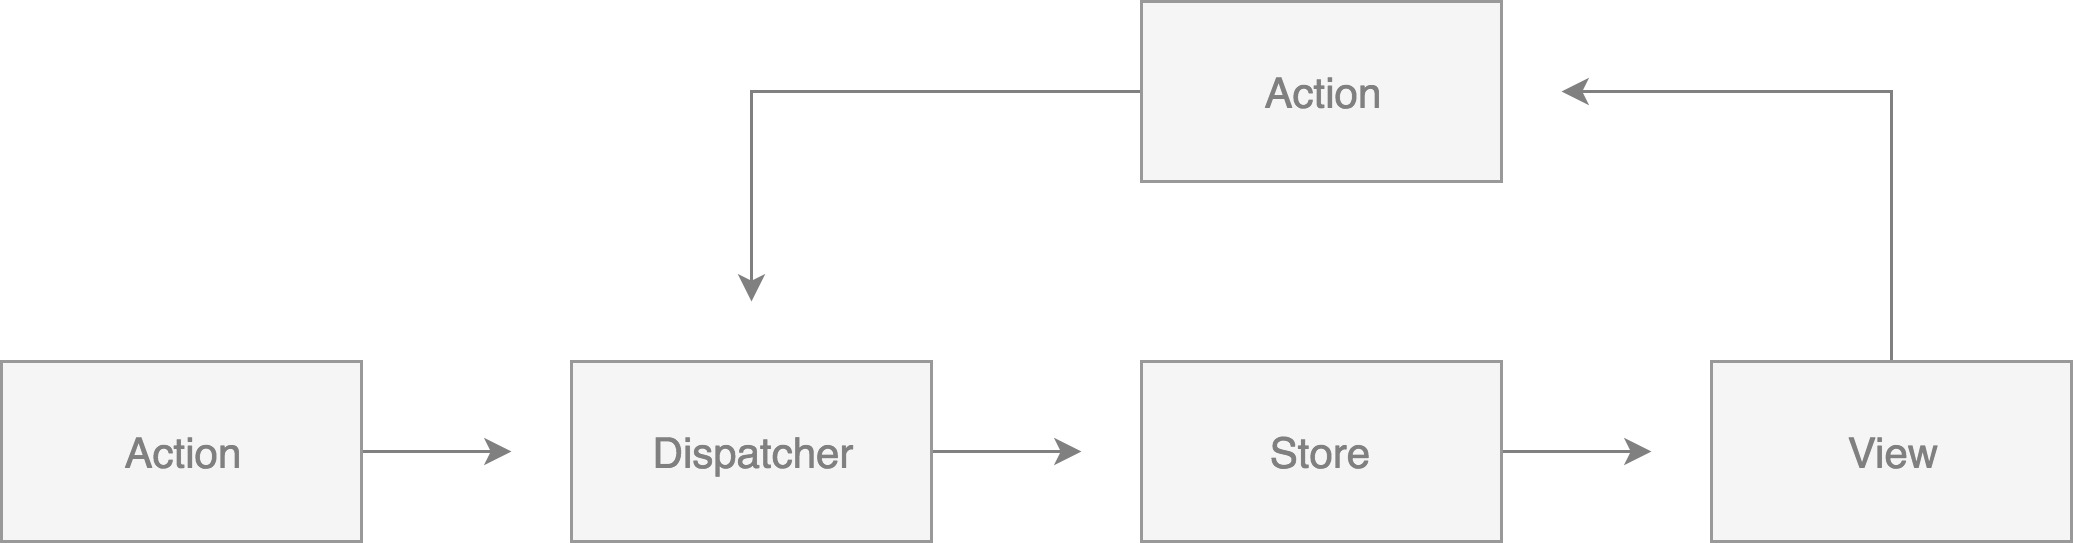
\includegraphics[width=14cm]{./images/FluxWorkflow}
\caption{Rappresentazione del flusso di dati con Flux.}
\label{FluxWorkflow}
\vspace*{0.5cm} 
\end{figure}

\noindent
In questa architettura la logica è divisa in due parti: ciò che riguarda gli eventi e le modifiche all'interfaccia è compreso nella View, la quale potrebbe essere definita una Controller-View in quanto esegue entrambi i lavori; la logica che riguarda invece lo stato dell'applicazione è compresa nello Store, i quali a seconda dell'azione eseguita si modificano di conseguenza.

